%----------------------------------------------------------------------------------------
%	PACKAGES AND OTHER DOCUMENT CONFIGURATIONS
%----------------------------------------------------------------------------------------

\documentclass[12pt]{article}



\usepackage[utf8]{inputenc} % Required for inputting international characters

\usepackage[T1]{fontenc} % Output font encoding for international characters

\usepackage[top=2cm,right=2cm, left=2cm]{geometry} % set margins

\usepackage{setspace} % paragraph spacing

\usepackage{mathpazo} % Palatino font


\usepackage{hyperref}  % for hyperlinks to resources\

\usepackage{graphicx} % for logo


\usepackage{pgfgantt} % for gantt chart


\usepackage{tabularx} % in the preamble
\newcolumntype{Y}{>{\centering\arraybackslash}X}
\newcolumntype{b}{>{\hsize=.5\hsize}X} % column 1 = 50% of a column
\newcolumntype{s}{>{\hsize=.4\hsize}X} % column 2 = 40% of a column
\newcolumntype{m}{>{\hsize=1.1\hsize}X} % column 3 = 110% of a column

\definecolor{barblue}{RGB}{153,204,254}
\definecolor{groupblue}{RGB}{51,102,254}
\definecolor{linkred}{RGB}{165,0,33}
\renewcommand\sfdefault{phv}
%\renewcommand\mddefault{mc}
%\renewcommand\bfdefault{bc}
\setganttlinklabel{s-s}{START-TO-START}
\setganttlinklabel{f-s}{FINISH-TO-START}
\setganttlinklabel{f-f}{FINISH-TO-FINISH}

\begin{document}

%----------------------------------------------------------------------------------------
%	TITLE PAGE
%----------------------------------------------------------------------------------------

\begin{titlepage} % Suppresses displaying the page number on the title page and the subsequent page counts as page 1
	\newcommand{\HRule}{\rule{\linewidth}{0.5mm}} % Defines a new command for horizontal lines, change thickness here
	
	\center % Centre everything on the page
	
	%------------------------------------------------
	%	Headings
	%------------------------------------------------
	
	\textsc{\LARGE University of Regina}\\[1.5cm] % Main heading such as the name of your university/college
	
	\textsc{\Large ENSE 477: Capstone Project}\\[0.5cm] % Major heading such as course name
	
	\textsc{\large Testing Strategy}\\[0.5cm] % Minor heading such as course title
	
	%------------------------------------------------
	%	Title
	%------------------------------------------------
	
	\HRule\\[0.4cm]
	
	{\huge\bfseries Telport: Sasktel Telecommunications Portal}\\[0.4cm] % Title of your document
	
	\HRule\\[1.5cm]
	
	%------------------------------------------------
	%	Author(s)
	%------------------------------------------------
	
	\begin{minipage}[t]{0.4\textwidth}
		\begin{flushleft}
			\large
			\textit{Authors}\\
			Dakota \textsc{Fisher}\\ % Your name
			200 344 336\newline \newline
			Quinn \textsc{Bast}\\ % Your name
			200 352 973
		\end{flushleft}
	\end{minipage}
	~
	\begin{minipage}[t]{0.4\textwidth}
		\begin{flushright}
			\large
			\textit{Supervisor}\\
			Dr. Yasser \textsc{Morgan} % Supervisor's name
		\end{flushright}
	\end{minipage}
	
	% If you don't want a supervisor, uncomment the two lines below and comment the code above
	%{\large\textit{Author}}\\
	%John \textsc{Smith} % Your name
	
	

%------------------------------------------------
	%	Logo
	%------------------------------------------------
		\vfill\vfill\vfill\vfill\vfill % Position the date 3/4 down the remaining page
	
\includegraphics[width=.5\textwidth]{UR_Logo_Primary_Full_Colour_RGB.jpg} % Include a department/university logo - this will require the graphicx package
	
	%------------------------------------------------
	%	Date
	%------------------------------------------------
	

	
	{Last Modified\\\large\today} % Date, change the \today to a set date if you want to be precise		

	
	 % Push the date up 1/4 of the remaining page
	 
	%----------------------------------------------------------------------------------------	
\end{titlepage}

%----------------------------------------------------------------------------------------


%----------------------------------------------------------------------------------------
% Revision History
%----------------------------------------------------------------------------------------
\section*{Revision History}
\begin{tabularx}{\textwidth}{|Y|Y|Y|}
\hline
  \textbf{Revision Version} & \textbf{Revision Author} & \textbf{Revision Date}\\
\hline
1.0 & Dakota Fisher & February 24, 2019 \\
\hline
\end{tabularx}

\newpage


%----------------------------------------------------------------------------------------
%	Table of Contents
%----------------------------------------------------------------------------------------

\pagestyle{plain} %get rid of header/footer for toc page
\pagenumbering{roman}

\tableofcontents %put Table of Contents in
\cleardoublepage %start new page

\listoffigures %put List of Figures in
\cleardoublepage %start new page

\listoftables %put List of Tables in
\cleardoublepage %start new page

\pagestyle{plain} % put headers/footers back on
\pagenumbering{arabic}

%----------------------------------------------------------------------------------------

%----------------------------------------------------------------------------------------
%	Body of Document
%----------------------------------------------------------------------------------------
%----------------------------------------------------------------------------------------
\doublespacing % set document to be default double spaced


%----------------------------------------------------------------------------------------
%	Introduction
%----------------------------------------------------------------------------------------

\section{Introduction}
\paragraph{}
	This document outlines and defines the Testing plan and libraries utilized to provide a stable, maintainable solution. The initial problem statement and proposed activities are suggestions given by Sasktel to provide a manageable scope. To provide a refresh on the intent of the project, the problem statement has been provided in the following paragraphs. The decisions on infrastructure, aside from the Broadworks API and telephone account access are left up to us to decide. 
\subsection{Problem Statement}
\paragraph{} 
	SaskTel requires a communications portal that can interwork with a Telephony Application Server and our core network to present communications and feature capabilities through a browser.  This will allow for the exploration of new communications service models. 
\paragraph{} 
	SaskTel has been pursuing the deployment of a new communications core along with the Cisco/Broadsoft Telephony Application Server branded as Broadworks.  One of the drivers is to enable a richer customer experience through a converged architecture that exposes rapid development to enables new capabilities.  Broadworks exposes the Application Programming Interface to access service control tools and user information.  These tools and information can be used to create new communications applications or add additional value to existing applications.  
\paragraph{} 
	The main objectives for SaskTel is to gain exposure to new and innovative communications service experience for our customers and to promote the potential internally for aligning resources, time and effort in enabling applications.

\section{Automated testing}
\paragraph{}	Testing is important for the project, and as such it needs to be done continuously. Plenty of tools exist to provide the frameworks and tools to create easily executed test frameworks. Namely there are tools that provide continuous integration testing, unit testing, and user experience testing. 

\subsection{TravisCI (In Use)}
\paragraph{}	TravisCI, completely referred to as Travis Continuous Integration is a cloud based testing service. It is Configured using a Yaml file to provide a configured Linux environment and run specified tests upon any merge request into the Master branch of the Github project. It provides a report, and if any tests fail it discourages the merge. There are alternatives such as CircleCI and Jenkins, but due to it's ease of use compared to Jenkins, and existing longer than CircleCI it was chosen for this project. The following figure demonstrates a passing test case, providing information on the build and test.
	\begin{figure}[h!]
	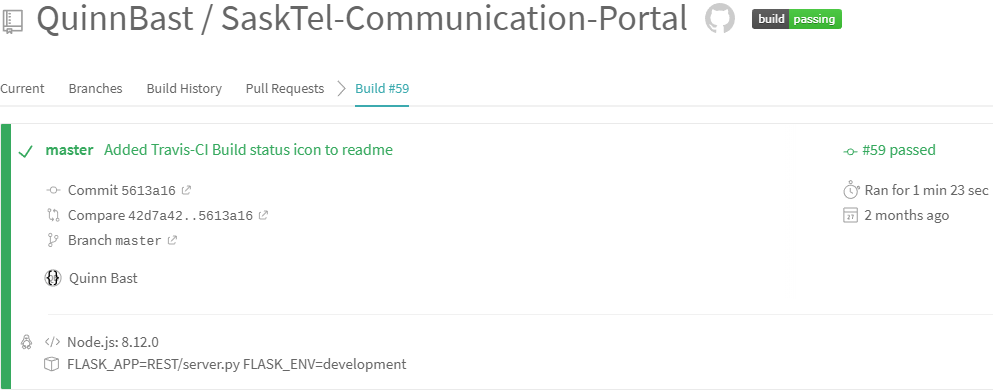
\includegraphics[width=\textwidth]{TravisCI.png}
	\caption{TravisCI Passing Build}
	\end{figure}
	\newpage

\subsection{Mocha (In Use)}
\paragraph{}	Mocha is a robust test bench, which provides a harness for running unit tests within a node JavaScript environment. The strengths of Mocha lay within it's ability to provide a framework for any nested javascript test library. Mocha can be used as a standalone solution, or with a medley of other test frameworks. The key combination of mocha test frameworks used in this project are Chai, Enzyme, and Sinon.
 
\subsection{Jest (Not In Use)}
\paragraph{}	 Jest is a similar solution to Mocha, and provides a very strong test framework foundation for test development. Jest is a slightly younger test library, and has slightly less community support compared to Mocha, and because of it's popularity, Mocha was chosen. Though, as test are developed, if Jest proves to be a stronger framework, it will be implemented accordingly. Jest also provides the ability to test code coverage. 
\subsection{Chai (In Use)}
\paragraph{}	Chai is a strong assertion library. It's vast reliability on asserting conditions and tests is pivotal to good test development. No matter what test framework. Chai is used in combination with Mocha to provide mocking and assertions for Mocha tests.
\subsection{Sinon (In Use)}
\paragraph{}	Sinon is a spy and stubbing framework in Javascript. The strengths of Sinon for this project are it's ability to mock server API's and endpoints as well as provide controlled bad data to monitor component responses.
\subsection{Enzyme (In Use)}
\paragraph{}	The test framework for React components, Enzyme, is a powerful rendering tool to test React components at all phases of it's life-cycle. Enzyme can incorporate many aspects of Sinon, and Chai to completely emulate controlled environments for each individual component.
\subsection{Selenium (In Use)}
\paragraph{}	Selenium is a browser automation testing tool. The benefits of using Selenium tests are that it lets user experience expectations be tested during each release, to make sure that the overall functionality using a mouse and keyboard are uninhibited. Being able to test that solutions are genuinely providing the correct user output is important. Tests can be completed on components, functions and classes, but unless the web page interacts as expected there's always some level of uncertainty in the test. 
\subsection{Cypress (Not In Use)}
\paragraph{}	Cypress is another browser emulation solution, similar to Selenium. The newly developed framework is a promising product, but at the time of creation of this project, it only supports testing in Chromium environments. Compared to Selenium's support for multiple browsers including Chromium, and Firefox. 
\subsection{NYC Istanbul (In Use)}
\paragraph{}	Istanbul, which is known as NYC in newer iterations, is a code coverage framework which spies on test frameworks such as Mocha to monitor and output test coverage. Every file touched by Mocha tests is analysed and reported on. 
\newpage

\section{User Stories}
\paragraph{}	The following sections denote common use cases for the program that we brainstormed and consider to be requirements by usability and basic principle. The basic structure for user stories is as follows. "As a <type of user> I would like to < be able to do task> so that I can < metric improvement to life>". User stories are referenced by the number following the chapter value, which means user story 1 will refer to sub-section x.1.

\paragraph{}	User stories are important for test development as they provide ground work for the requirements and functionalities that tests should be sure to incorporate and provide solutions for. The following user stories are utilized to provide a feature driven development approach to the project, while keeping quantifiable, and testable data present to be monitored during development. 

\subsection{Log In}
\paragraph{}	As a \textit{SaskTel Customer}, I would like to be able to \textit{Log into the program} so that I can \textit{use the program and check my information}.

\subsection{Log Out}
\paragraph{}	As a \textit{SaskTel Customer}, I would like to be able to \textit{Log out of the program} so that I can \textit{ensure that anyone using my computer can't access my account}.

\subsection{Check Call Logs}
\paragraph{}	As a \textit{SaskTel Customer}, I would like to be able to \textit{check my call logs} so that I can \textit{check when I got calls, and see who called me/when}.

\subsection{Turn on Call Forwarding Always}
\paragraph{}	As a \textit{SaskTel Customer}, I would like to be able to \textit{always forward calls sent to my phone} so that I can \textit{answer them on my main phone and not worry about my secondary phone}.

\subsection{Turn on Call Forwarding Busy}
\paragraph{}	As a \textit{SaskTel Customer}, I would like to be able to \textit{forward calls when my phone is busy} so that I can \textit{feel comfortable that those calling me get sent to someone who can answer}.

\subsection{Turn on Call Forwarding Selective}
\paragraph{}	As a \textit{SaskTel Customer}, I would like to be able to \textit{forward phone calls to another phone during a scheduled time} so that I can \textit{so that phone calls can be forwarded when I have planned events in the way of answering my phone}.

\subsection{Turn on Call Forwarding No Answer}
\paragraph{}	As a \textit{SaskTel Customer}, I would like to be able to \textit{forward calls when I'm away from my phone} so that I can \textit{answer them on my cell phone when I'm away from my land line}.

\subsection{Turn on Call Forwarding}
\paragraph{}	As a \textit{SaskTel Customer}, I would like to be able to \textit{forward phone calls to another number} so that I can \textit{be sure that important calls reach me on my cell phone or work phone}.

\subsection{Turn on Do Not Disturb}
\paragraph{}	As a \textit{SaskTel Customer}, I would like to be able to \textit{decline all calls to my phone number} so that I can \textit{have some time without worrying about phone calls interrupting me}.

\subsection{View my Profile}
\paragraph{}	As a \textit{SaskTel Customer}, I would like to be able to \textit{view my account information} so that I can \textit{know that I am using the right account}.

\subsection{Call a Phone Number}
\paragraph{}	As a \textit{SaskTel Customer}, I would like to be able to \textit{call a phone number from my computer} so that I can \textit{easily make phone calls without using my phone}.

\subsection{Start a Call to a Phone Number from my Phone}
\paragraph{}	As a \textit{SaskTel Customer}, I would like to be able to \textit{call another phone number from my phone} so that I can \textit{more easily call phone numbers I find on my computer}.

\subsection{View Feature Access Codes}
\paragraph{}	As a \textit{SaskTel Customer}, I would like to be able to \textit{check what star codes I can use} so that I can \textit{understand what I can do with my phone when I can't log into the application}.




\newpage
\section{Tests}
\paragraph{}	As test cases are created, and audited to be successful test cases they're documented in this section. In order to have a record trail of the tested features and tests that are required, during the test development phase of our project, the following sections will begin to be fleshed out in further detail.

\subsection{Unit}
\paragraph{}	This section consists of all test cases that test JavaScript functions and classes.
\subsubsection{Login Page}
\begin{enumerate}	
	\item The login page must have the following components:
	\begin{enumerate}
		\singlespacing
		\item Phone Number Field
		\item Password Field
		\item Login button
	\end{enumerate}
	\item The login page must provide feedback on invalid input:
	\begin{enumerate}
		\singlespacing
		\item Incomplete or incorrect Phone Number
		\item Empty Password field, as the requirements are undefined
		\item Login button with invalid Phone Number or password, pre-auth attempt
		\item Invalid login response to auth attempt
	\end{enumerate}
\end{enumerate}	
\newpage
\subsection{User Experience} 
\paragraph{}	This section consists of all test cases that tests the complete website against simulated user scenarios and tests expected behaviours.
\subsubsection{Login}
\begin{enumerate}	
	\item The login page must respond to user input in the following inputs:
	\begin{enumerate}
		\singlespacing
		\item Phone Number Field
		\item Password Field
		\item Login button
	\end{enumerate}
	\item The login attempts must provide feedback on invalid input:
	\begin{enumerate}
		\singlespacing
		\item Incomplete or incorrect Phone Number
		\item Empty Password field, as the requirements are undefined
		\item Login button with invalid Phone Number or password, pre-auth attempt
		\item Invalid login response to auth attempt
	\end{enumerate}
		\item The Phone number field must:
	\begin{enumerate}
		\singlespacing
		\item Only allow digits to be entered
		\item provide a guide for the user to follow
		\item Explain the requirements for the phone number
	\end{enumerate}
	\item The page must redirect to the Application main page upon successful login.
\end{enumerate}	
\newpage
\subsection{Component}
\paragraph{}	This section consists of all test cases that test React Components state rendering and life-cycle correctness.
\subsubsection{Login UX}
\begin{enumerate}	
	\item The Login component must:
	\begin{enumerate}
		\singlespacing
		\item Track the entered phone number in state
		\item Track the entered password in state
		\item communicate with the auth component
	\end{enumerate}
	\item The login page must provide feedback on invalid input:
	\begin{enumerate}
		\singlespacing
		\item Incomplete or incorrect Phone Number
		\item Empty Password field, as the requirements are undefined
		\item Login button with invalid Phone Number or password, pre-auth attempt
		\item Invalid login response to auth attempt
	\end{enumerate}
\end{enumerate}	








\end{document}

%----------------------------------------------------------------------------------------
%	Document Style Templates
%----------------------------------------------------------------------------------------
%%%%%%%%%%%%%%%%%%%%%%%%%%%%%%%%%%%%%%%%%
% Section Nesting for Table of Contents
%
% A section or subsection can contain any number of nested children
%
%%%%%%%%%%%%%%%%%%%%%%%%%%%%%%%%%%%%%%%%%
% \section{First Title} %x
% \paragraph{} **~ Contents of First Title ~**
%
% \subsection{Second Title} %x.x
% \paragraph{} **~ Contents of Second Title ~**
%
% \subsubsection{Third Title} %x.x.x
% \paragraph{} **~ Contents of Third Title ~**
% 
% No more nesting allowed. capped at x.x.x sectioning
%
%
%%%%%%%%%%%%%%%%%%%%%%%%%%%%%%%%%%%%%%%%%
%
%----------------------------------------------------------------------------------------

%----------------------------------------------------------------------------------------
%	Template References and Licenses
%----------------------------------------------------------------------------------------
% This paper integrates the following templates into a single document.
% There is no endorsement in any way shape or form from the template authors.
%
%%%%%%%%%%%%%%%%%%%%%%%%%%%%%%%%%%%%%%%%%
% Academic Title Page
% LaTeX Template
% Version 2.0 (17/7/17)
%
% This template was downloaded from:
% http://www.LaTeXTemplates.com
%
% Original author:
% WikiBooks (LaTeX - Title Creation) with modifications by:
% Vel (vel@latextemplates.com)
%
% License:
% CC BY-NC-SA 3.0 (http://creativecommons.org/licenses/by-nc-sa/3.0/)
% 
%
%%%%%%%%%%%%%%%%%%%%%%%%%%%%%%%%%%%%%%%%%
